\documentclass[a4paper,twocolumn]{scrartcl}

\usepackage{graphicx}
%\usepackage{hyperref}
\usepackage{url}


%% Limit: 40000 chars
%% check with `detex paper.tex | wc -m`

\title{DNSKEY Management}
\author{Julien Perrochet \and Tobias Schlatter}
\date{December 12, 2012}

\graphicspath{{../figures/}}

\newcommand{\wbjp}{\protect\footnote{Written by Julien Perrochet}}
\newcommand{\wbts}{\protect\footnote{Written by Tobias Schlatter}}


\begin{document}

\maketitle

\section{Introduction}
%% TODO add some blah about management and penetration.

In the following, every necessary operation for key management in
DNSSEC is described as a reminder to the reader.

\paragraph{Enabling DNSSEC} When enabling DNSSEC for a zone, the
parent zone has to establish and sign a DS record with the newly
created public-key.

\paragraph{Key Rollover} RFC4641 \cite{RFC4641} suggests that the DNSKEY
records for a zone should be changed somewhere between once every week
up to once every month. While the detailed rollover procedure is
irrelevant here, it is important to know, that the parent zone has to
update the its DS record.

\paragraph{Disabling DNSSEC} An operator might choose to discontinue
DNSSEC for a zone. The DS records (or other means of signing DNSKEYs
as we will see later) need to be removed.

\section{DNSSEC Deployment\wbts}

This section will expose the current deployment status of DNSSEC and
give the reader an idea about the current DNSSEC landscape before
going into the specific DNSKEY management issues. Please refer to
section~\ref{sec:case-study} for more details on the situation of the
\verb|ch.| zone.

\subsection{Penetration in Production}
In figure~\ref{fig:dnssec-growth} you can see the development of
deployed, production DNSSEC zones. The data comes from SecSpider
\cite{secspider} which crawls as many DNSSEC zones as possible,
verifies whether it is properly signed and then applies a heuristics to
determine whether it is actually a production zone. The goal is to
rule out zones which are created for testing such as
\url{bogussig.bogussig.test.jelte.nlnet.labs.nl}.

We can see that DNSSEC is gradually being deployed and the number of
signed production zones grows rapidly (note the log-scale!). The rapid
increase of crawled DNSSEC zones mid-2008, so interprets
\cite{Osterweil09}, is due to a cache poisoning attack discovered in
summer 2008 \cite{dnsVuln}. During our research, we were unfortunately
unable to find an estimate of the number of (production) DNS zones in
the Internet to estimate the percentage of DNSSEC penetration.

Contrary to the state at writing of \cite{Osterweil09}, the DNS
root-zone is signed since July 15, 2010 \cite{root-dnssec} and hence
serves as the global trust anchor. However, as of this writing,
data\footnote{\url{http://secspider.cs.ucla.edu/islands.html}}
gathered by \cite{secspider} suggests that more than half of the
deployed DNSSEC zones which are verifiable (i.e. are likely not to
have a spoofed key, see SecSpider in the next section or
\cite{Osterweil09} for details), do not have a fully linked
certificate chain up to the root zone.

\begin{figure*}
  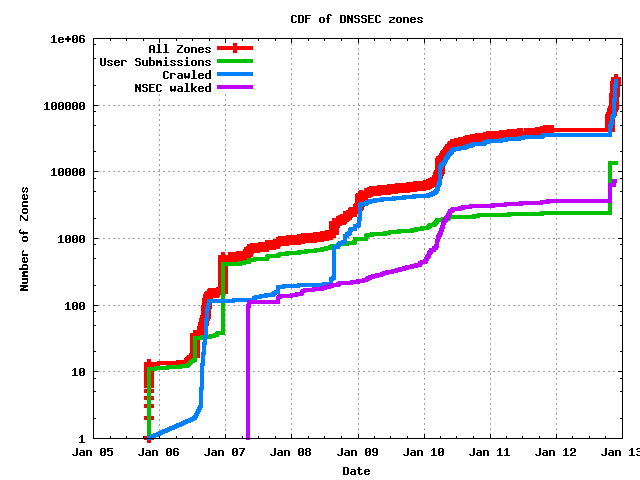
\includegraphics[width=\linewidth]{dnssec-growth}
  \caption{Number of deployed DNSSEC zones by
    SecSpider \cite{secspider}}
  \label{fig:dnssec-growth}
\end{figure*}

\subsection{Trust Anchor Repositories}
Not always can the certificate chain be ensured from the root-zone
down to a DNSSEC zone. Before the signing of the root-zone, it was
obviously impossible to do such a thing, after the signing -- as
formerly discussed data suggests -- there are still orphaned zones
whose parent isn't properly signed.

A Trust Anchor Repository (TAR) can be used in such a situation to
supply resolvers with the trusted public key for a given zone during
DNS resolution, therefore the name \emph{inline repository}. One of
these repositories is the Interim Trust Anchor Repository (ITAR)
formerly operated by IANA and discontinued since the signing of the
root-zone \cite{itar}.

The Internet Software Consortium (ISC) still runs an inline TAR
\cite{iscDlv}, using the DNSSEC Lookaside Validation standard
\cite{RFC5074}. When a resolver needs to check the key of a zone
\verb|<X>| with this TAR, it makes a DNS request of type DLV to 
\url{<X>.dlv.isc.org}. If it succeeds, the DLV record contains the
signature for the (hopefully matching) DNSKEY. The ISC inline TAR
requires manual addition of keys to the repository.

SecSpider \cite{secspider, Osterweil09} is another inline TAR, but
uses a different approach for key validation: Rather then entering and
signing public keys manually, it randomly queries DNSKEY entries from
different point in the world simultaneously and only enters it into
the TAR, if all the received keys match. This makes spoofing of a key
very difficult due to the spatial distribution and the
unpredictability of the queries.

Another type of TAR resides at the resolver: A statically configured
TAR stores keys locally at the resolver and hence needs not to issue an
additional query for keys when a new DNS request arrives. The
statically configured TAR may automatically poll keys asynchronously,
or is maybe just a bunch of manually configured trusted keys. As an
example of a statically configured TAR, we have
Vantages\footnote{\url{http://www.vantage-points.org/}}, an addition
to a standard resolver, \cite{Osterweil09} which can poll keys from
different locations such as web pages, but also also other
vantage-enabled resolvers. Of course, the operator may also choose to
add trusted keys manually.

\section{Operations\wbjp}
\subsection{3Rs}
%% Talk about EPP or push burden to Case-Study
\subsection{Single admin}
\subsection{Multi admin}
\subsection{Disabling}

\section{Case-Study: Switzerland (\texttt{ch.} Zone)\wbts}
\label{sec:case-study}

\paragraph{Certificate Chain} According to a query on
\cite{secspider}, the \verb|ch.| TLD zone is signed and fully
verifiable from the root zone anchor on downwards. The certificate
chain can hence fully be established and no separate TAR is required.

\paragraph{Penetration} SWITCH states on their website that as of
30. September 2012, 1'734'170 child-zones of \verb|ch.| have been
registered\footnote{\url{https://www.nic.ch/reg/cm/wcm-page/statistics/index.html}}. Upon
inquiry, SWITCH stated that there are around 370 secure delegations
from the \verb|ch.| zone. This is less than $0.02\%$ penetration
rate.

\paragraph{Key Management} The validity period of a zone signing key
(for \verb|ch.|) is 37 days \cite{switch10}. For child zones,  DNSSEC
and DNSKEY entries can be enabled and disabled through SWITCH's 
web-interface which is able to pull the keys automatically from the
authoritative DNS servers. Partners (as Registrars are called in
Switzerland) may also use EPP for key rollover.

Therefore, it is relatively simple to enable DNSSEC for a \verb|<X>.ch.| 
zone. While using the web-interface is certainly cumbersome when
having to deal with rollovers for a large number of domains, any major
provider may become a SWITCH Partner and can then switch over to EPP
which solves this issue.

\nocite{*}
\bibliographystyle{abbrv}
\bibliography{dnssec}

\end{document}

%%% Local Variables: 
%%% mode: latex
%%% TeX-master: t
%%% End: 
